\section{Introduction}

Variety of applications need a lower dimensional, concise and faithful representation of the original parent geometry. A skeleton is such an entity which represents shape of it's parent object. It being simpler than the parent object, applications like pattern recognition, approximation, similarity estimation, collision detection, animation, matching and deformation can be performed efficiently on it than on the parent object. 

Approaches such as Medial Axis Transform (MAT),  Chordal Axis Transform (CAT), Thinning etc. are used to compute skeletons. Table \ref{Medials} briefly summarizes some of these along with their strengths-weaknesses. In this paper terms like 'Skeleton', 'Midcurve' and 'Medial' are used synonymously, unless otherwise specified.

\begin{table}
\caption{Current Medial Computation Methods}
\begin{tabular}[h]{@{} p{0.14\linewidth}  p{0.22\linewidth}  p{0.22\linewidth}  p{0.23\linewidth} @{}} \toprule
{\bf Method } & {\bf Medial }  & {\bf Description} & {\bf Problems}\\
\midrule
%------------------------------------------------------------------------------------------------------------------------------------
\raisebox{-.9\height}{MAT \cite{Ramanathan2004}} &
\raisebox{-.9\height}{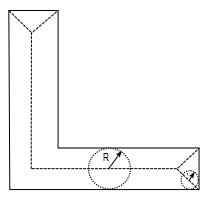
\includegraphics[scale=0.3]{..//Common/images/MAT.png} }&
Locii of centers of maximal disk &
Unwanted branches. \\


%------------------------------------------------------------------------------------------------------------------------------------
\raisebox{-.9\height}{CAT \cite{Quadros2008}}&
\raisebox{-.9\height}{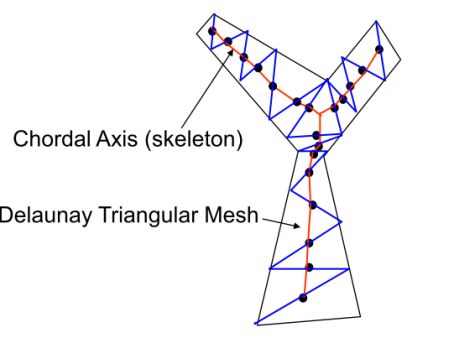
\includegraphics[scale=0.45]{..//Common/images/CAT.png}}&
Triangulation. Joins midpoints  &
Gaps at end. Expensive triangulation. \\


%------------------------------------------------------------------------------------------------------------------------------------
{Straight Skeleton \cite{Henrik2004}} &
\raisebox{-.9\height}{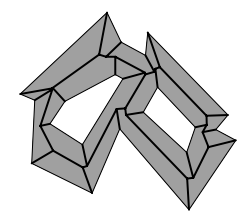
\includegraphics[scale=0.28]{..//Common/images/Straight.png}} &
Thinning from boundary. &
Bisectors not equidistant.\\

\bottomrule
\end{tabular}
\label{Medials}
\end{table}


This paper focuses on 2D planar sketch profiles (with an assumption that curved shapes can be converted to polygonal shape by faceting). Divide-and-Conquer has been used where Decomposition partitions the given shape into sub-shapes and then Skeletonization creates midcurves in simpler sub-polygons.  At the end, individual midcurves are extended-joined to form a continuous set of curves mimicking the parent shape.
